\chapter{Influence Diagrams}
\label{ch-influ-diag}

This chapter is based on Refs.\cite{sha-influ-diag}
and \cite{limid-one}.


An {\bf Influence Diagram (ID)} is
a DAG that generalizes a bnet by adding
2 new types of nodes. IDs have 3 types of nodes: chance, decision and utility (a.k.a value) nodes, represented, respectively, by ovals, squares and diamonds. Table \ref{tab-id-nodes} compares these 3 types of nodes.

% Please add the following required packages to your document preamble:
% \usepackage[table,xcdraw]{xcolor}
% Beamer presentation requires \usepackage{colortbl} instead of \usepackage[table,xcdraw]{xcolor}
\begin{table}[h!]
\begin{tabular}{|l|l|l|l|}
\hline
                                                                                            & \cellcolor[HTML]{FFFFC7}\begin{tabular}[c]{@{}l@{}}Chance node \\ (oval)\end{tabular} & \cellcolor[HTML]{FFFFC7}\begin{tabular}[c]{@{}l@{}}Decision node\\ (square)\end{tabular} & \cellcolor[HTML]{FFFFC7}\begin{tabular}[c]{@{}l@{}}Utility node\\ (diamond)\end{tabular} \\ \hline
\cellcolor[HTML]{FFFFC7}type of states                                                      & discrete                                                                     & discrete, binary usually                                                                       & continuous                                                                             \\ \hline
\cellcolor[HTML]{FFFFC7} deterministic?                                                   & Not in general                                                                        & Yes                                                                                      & Yes                                                                                    \\ \hline
\cellcolor[HTML]{FFFFC7}transition info\footnote{by ``transition info" of a node, we
mean ``personal" node info
other than a list of the states of the node and a list 
of its parent nodes}                                                    & TPM                                                                                   & 
deterministic TPM                                                                                 & utility function                                                                       \\ \hline
\cellcolor[HTML]{FFFFC7}children type                                                       & chance, decision, value                                                               & chance, decision, value                                                                  & None                                                                                   \\ \hline
\cellcolor[HTML]{FFFFC7}\begin{tabular}[c]{@{}l@{}}can be fixed\\ by observer?\end{tabular} & Yes                                                                                   & Yes                                                                                      & No                                                                                     \\ \hline
\end{tabular}
\caption{Comparison of the 3 types
of nodes in an influence diagram.
The only difference between chance and 
decision nodes is that chance nodes have
a probabilistic TPM and decision nodes have
a deterministic one.}
\label{tab-id-nodes}
\end{table}
Let

$\rvc.=$ set of {\bf chance nodes}

$\rvd.=$ set of {\bf decision nodes}
Assume $\rvd_i$ are in chronological
order, i.e., $\rvd_i$ occurs before $\rvd_{i+1}$ for all $i$.

$\rvu.=$ set of {\bf utility nodes}. Often, utility nodes are called {\bf value nodes} and only their sum is called a utility node.

$\rvX.= \rvc. \cup \rvd. \cup \rvu.$ all nodes

$\rve.=$ {\bf evidence nodes}, the subset $\rve.$  of the chance nodes $\rvc.$ that is {\bf apriori observed}
(i.e. measured before the experiment starts). If a decision node has a 
chance node as a parent,
we will assume it is measured immediately before the decision is made,
not apriori.


$u_i(pa(\rvu_i))=$ {\bf partial utility function}

$u(\rvc., d.)=\sum_i u_i(pa(\rvu_i))$ {\bf total utility function }

\begin{itemize}


\item{\bf Optimal Strategy}

Let
\beq
L_i = \lim_{pa(d_i)\rarrow pa(d_i)^*}
\eeq
for $i=1,2, \ldots, nd$.
Next let



\beq
pa(d_1)^* = \argmax_{pa(d_1)}E_{\rvc.-pa(\rvd_1)}[u(\rvc., d.)]
\eeq


\beq 
pa(d_2)^* = \argmax_{pa(d_2)}L_1E_{\rvc.-pa(\rvd_1)-pa(\rvd_2)}[u(\rvc., d.)]
\eeq

\beq 
pa(d_3)^* = \argmax_{pa(d_3)}L_2 L_1 E_{\rvc.-pa(\rvd_1)-pa(\rvd_2)-pa(\rvd_3)}[u(\rvc., d.)]
\eeq
and so on for $pa(d_i)^*$ for $i=1,2, \ldots, nd$.

Note that $\max_{pa(d_i)} = \max_{d_i}$
because $d_i=d_i(pa(d_i)) $ where
$d_i()$ is a smooth deterministic function.

Define $d_i^*$ by

\beq
d_i^* = d_i(pa(d_i)^*)
\eeq


\item {\bf Expected Utility}
\beq
EU(d.)=E_{\rvc.}[u(\rvc., d.)]=
\sum_{c.} P(c.)u(c., d.)
\eeq
where 
\beq
P(c.)= P(c.-e.)\delta(e., e.')
\eeq
or
\beq
P(c.)= P(c.-e.-y.)\delta(e., e.')\delta(y., y^*)
\eeq
where 
\beq 
y^*.= \cup_{i=1}^{nd}pa(d_i)^*
\eeq


\item {\bf Maximum Expected Utility}

\beq
MEU=EU(d.^*)
\eeq
where $d.^*$ is the optimal strategy.


\item {\bf Limited Memory ID (LIMID)}. 

LIMIDs were first introduced 
in Ref.\cite{limid-one}. According to that reference, LIMIDs are ``multistage decision problems in which the traditional assumption of no forgetting is
relaxed." 
Note that ``multistage decision problems" is another term
for a dynamic bnet (see Chapter \ref{ch-dyn-bnets}).

Here is an example of LIMIDs.
Figs.\ref{fig-pre-limid} and \ref{fig-post-limid}
come from Ref.\cite{limid-one} and describe pig farming
at various times $T=\{1,2,3,4\}$.

Node $\rvh_i\in\bool$
refers to the health of a pig at time $i$.

Node $\rvt_i\in \bool$ refers to a test 
conducted on the pig at time $i$.

Node $\rvd_i\in \bool$ refers to a decision 
made by the farmer at time $i$ on whether to medicate the pig.

Node $\rvu_i\in \RR$ refers to the utility (monetary value)  
of medicating the pig at time $i$.

 
Fig.\ref{fig-pre-limid} shows a dynamic bnet that
obeys the {\bf no forgetting} assumption so every decision is
privy to the state of all previous decision and chance nodes.
Fig.\ref{fig-post-limid} shows the same bnet as 
Fig.\ref{fig-pre-limid} after all arrows entering a decision $\rvd_i$ and originating at an earlier time, have been removed.



\begin{figure}[h!]
\centering
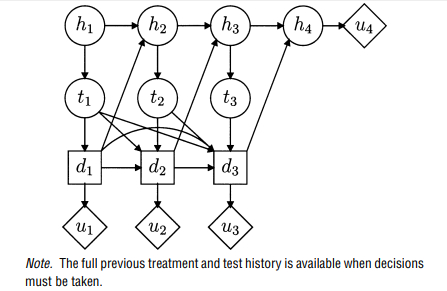
\includegraphics[width=4in]
{influ-diag/pre-limid.jpg}
\caption{Pig farming ID that obeys the ``no-forgetting"
assumption.  
}
\label{fig-pre-limid}
\end{figure}


\begin{figure}[h!]
\centering
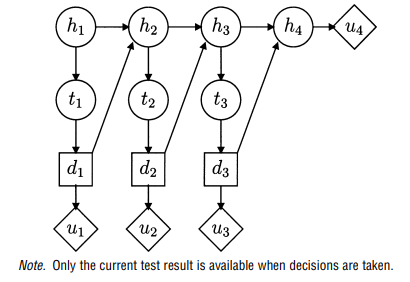
\includegraphics[width=4in]
{influ-diag/post-limid.jpg}
\caption{Pig farming ID that obeys the  LIMID
assumption. This ID is the same as the ID of Fig.\ref{fig-pre-limid},
except that the arrows pointing to a decision and originating at a previous time, have been removed.}
\label{fig-post-limid}
\end{figure}

\item {\bf Finding optimal strategy }


Ref.\cite{sha-influ-diag} proposes the following 3 exact methods for
finding the optimal strategy, EU and MEU of an ID.
\begin{enumerate}
\item conversion to a decision
tree 
\item calculation directly from ID, using Variable
Elimination Algorithm (VEA)
\item conversion to a rooted cluster tree.
\end{enumerate}

All 3 methods require  reversing some arrows. To reverse
an arrow, $\rvx\rarrow \rvy$, we add dummy arrows going into $\rvx$ or into
$\rvy$ so that $pa(\rvx)=pa(\rvy)= \calc$. After that, we use Bayes rule conditioned on $\calc$.


\beq
P(x|y, \calc) = \frac{P(y|x, \calc)P(x|\calc)}{\sum_x \text{ numerator}}
\eeq




In the next section,
we discuss method 2 (VEA).

\end{itemize}

\section{Variable Elimination Algorithm (VEA)}


VEA utilizes the following operations:
\begin{enumerate}
\item Summing over barren (i.e., childless) chance nodes.
\item Reversing $\rvx\rarrow \rvy$
to $\rvy\rarrow \rvx$
using Bayes Rule.
\beq
\xymatrix{
\corchete{a.}\ar[d]
&\corchete{b.}\ar[dl]\ar[dr]
&\corchete{c.}\ar[d]
\\
x\ar[rr]&&y
}
\xymatrix{\\\text{\;\;equals\;\;}}
\xymatrix{
\corchete{a.}\ar[d]\ar[drr]
&\corchete{b.}\ar[dl]\ar[dr]
&\corchete{c.}\ar[d]\ar[dll]
\\
x&&y\ar[ll]
}
\eeq

\item Summing over the states of a chance node. Suppose
$\rvx\rarrow \rvu$ 
where $\rvx$ is a chance node and $\rvu$
is a utility node, and $\rvx$ has only one child $\rvu$. Then
\beq
\xymatrix{
\corchete{a.}\ar[d]
&\corchete{b.}\ar[dl]\ar[dr]
&\corchete{c.}\ar[d]
\\
x\ar[rr]
&&\diamante{u}
}
\xymatrix{
&\implies&
\\
&\sum_x&}
\xymatrix{
\corchete{a.}\ar[drr]
&\corchete{b.}\ar[dr]
&\corchete{c.}\ar[d]
\\
&&\diamante{u}
}
\eeq

\item Finding state of decision node that maximizes utility. 
Suppose $\rvd\rarrow \rvu$ 
where $\rvd$ is a decision node and $\rvu$
is a utility node, and $\rvd$ has only
one child $\rvu$. Also
$\rva.\cup\rvb.=pa(\rvd)\supset pa(\rvu)=\rvb.$. So the 
maximization is $\max_du (d(b., a.), b.)$.
The value $d^*=\argmax_d u$
should ve saved.

\beq
\xymatrix{
\corchete{a.}\ar[d]
&\corchete{b.}\ar[dl]\ar[dr]
&
\\
\cuadro{d}\ar[rr]
&&\diamante{u}
}
\xymatrix{&\implies&
\\
&\max_{d} &}
\xymatrix{
\corchete{a.}
&\corchete{b.}\ar[dr]
&
\\
&&\diamante{u}
}
\eeq

\item Combining partial
utilities. 
\beq
\xymatrix{
\corchete{a.}\ar[d]
&\corchete{b.}\ar[dl]\ar[dr]
&\corchete{c.}\ar[d]
\\
\diamante{u_1}\ar[rr]
&&\diamante{u_2}
}
\xymatrix{\\\text{\;\;equals\;\;}}
\xymatrix{
\corchete{a.}\ar[drr]
&\corchete{b.}\ar[dr]
&\corchete{c.}\ar[d]
\\
&&\diamante{u_1 +u_2}
}
\eeq
\end{enumerate}

VEA consists of the 
the following steps applied in non-sequential
order. VEA is valid for even if
non-forgetting is assumed.

\begin{enumerate}

\item If there is a barren chance node
$\rvc$, sum over it.

\item
If $\rvd\rarrow \rvu$ where $\rvd$
is a decision node 
and $\rvu$ is a utility node, and $\rvd$ has exactly one child $\rvu$, and all $pa(\rvu)-\rvd$ have been
observed already, find $\max_d$ and remove $\rvd$.

\item If $\rvc\rarrow\rvu$,
where $\rvc$ is a chance node
and $\rvu$ is a utility node, and $\rvc$ has at most one child, then, after reversing arcs to its 
non-utility children in reverse chronological order,
sum over $\rvc$ and remove it.

\item Merge utility nodes $\rvu_1$ and $\rvu_2$,
preferably when $pa(\rvu_1)\subset pa(\rvu_2)$.



\end{enumerate}

We end this section with an example of VEA.\footnote{
Note that the nodes of these IDs
are not underlined. This is intentional.
Rather than representing a
network of abstract random variables,
they represent an instantiation of that network.  (see Chapter \ref{ch-bnet-def})}

\beq
\xymatrix@R=1pc@C=.5pc{
a\ar[dr]
&&&&
\cuadro{d_4}\ar[ddr]
&
\\
&c\ar[dr]
&&g\ar[drr]\ar[ur]
\\
b\ar[dr]\ar[ur]\ar[dd]
&&e\ar[dr]\ar[ur]
&&&\diamante{u_2}
\\
&d\ar[dr]\ar[ur]
&&\cuadro{d_2}\ar[uuur]\ar[urr]
\\
\cuadro{d_1}\ar[dr]\ar[ur]
&&f\ar[dr]\ar[rrr]
&&&\diamante{u_3}
\\&\diamante{u_1}
&&\cuadro{d_3}\ar[urr]\ar[rr]
&&\diamante{u_4}
}
\xymatrix{\\\\&
\implies&
\\
&\max_{d_4} &}
\xymatrix@R=1pc@C=.5pc{
a\ar[dr]
&&&&
&
\\
&c\ar[dr]
&&g\ar[drr]
\\
b\ar[dr]\ar[ur]\ar[dd]
&&e\ar[dr]\ar[ur]
&&&\diamante{u_2}
\\
&d\ar[dr]\ar[ur]
&&\cuadro{d_2}\ar[urr]
\\
\cuadro{d_1}\ar[dr]\ar[ur]
&&f\ar[dr]\ar[rrr]
&&&\diamante{u_3+u_4}
\\&\diamante{u_1}
&&\cuadro{d_3}\ar[urr]
&&
}
\eeq

\beq
\xymatrix{\\\\
\implies&
\\
{\scriptstyle \max_{d_3} \sum_g}&
}
\xymatrix@R=1pc@C=.5pc{
a\ar[dr]
&&&&
&
\\
&c\ar[dr]
&&
\\
b\ar[dr]\ar[ur]\ar[dd]
&&e\ar[rr]\ar[dr]
&&\diamante{u_2}
\\
&d\ar[dr]\ar[ur]
&&\cuadro{d_2}\ar[ur]
\\
\cuadro{d_1}\ar[dr]\ar[ur]
&&f\ar[rr]
&&\diamante{\scriptstyle
u_3+u_4}
\\&\diamante{u_1}
}
\xymatrix{\\\\
\implies&
\\
\scriptstyle
\max_{d_2}\sum_f&}
\xymatrix@R=1pc@C=.5pc{
a\ar[dr]
\\
&c\ar[dr]
\\
b\ar[dr]\ar[ur]\ar[dd]
&&e\ar[r]
&\diamante{u_2}
\\
&d\ar[dr]\ar[ur]
\\
\cuadro{d_1}\ar[dr]\ar[ur]
&&\diamante{
\scriptstyle
u_3+u_4}
\\&\diamante{u_1}
}
\eeq

\beq
\xymatrix{
\implies&
\\
\scriptstyle
\sum_{a,c, e}P(a)&}
\xymatrix@R=1pc@C=.8pc{
b\ar[rr]\ar[dr]\ar[dd]
&&\diamante{u_2}
\\
&d\ar[ur]\ar[r]
&\diamante{u_3+u_4}
\\
\cuadro{d_1}\ar[rr]\ar[ur]
&&\diamante{u_1}
}
\xymatrix{
\implies&
\\
\text{merge}
}
\xymatrix@R=1pc@C=.8pc{
b\ar[rr]\ar[dr]\ar[dd]
&&\diamante{\sum_{i=2,3,4}u_i}
\\
&d\ar[ur]
\\
\cuadro{d_1}\ar[rr]\ar[ur]
&&\diamante{u_1}
}
\eeq

\beq
\xymatrix{
\implies&
\\
\sum_d&}
\xymatrix@R=1pc@C=.8pc{
b\ar[r]\ar[d]
&\diamante{\sum_{i=2,3,4}u_i}
\\
\cuadro{d_1}\ar[r]\ar[ur]
&\diamante{u_1}
}
\xymatrix{
\implies&
\\
\text{merge}
}
\xymatrix@R=1pc@C=.8pc{
b\ar[r]\ar[d]
&\diamante{\sum_{i=1,2,3,4}u_i}
\\
\cuadro{d_1}\ar[ur]
}
\eeq


\beq
\xymatrix{
\\
\stackrel{\implies}{\max_{d_1}}&}
\xymatrix{
\\
b\ar[r]
&\diamante{\sum_{i}u_i}
}
\xymatrix{
&&
\\
&\stackrel{\implies}{
\scriptstyle
\sum_b P(b)}}
\xymatrix{
\\
\diamante{\sum_{i}u_i}
}
\eeq






%\section{Conversion to Tree}
%Finding the optimal strategy 
%for an ID with discrete chance and decision nodes is basically
%a problem of finding a list of possible instantiations
%for the parents of each decision node, and finding the
%instatiation that maximizes each each utility function.
%Trees are eminently suited for generating lists of
%possibilities.
%
%We begin by assigning each  chance node
%of Fig.\ref{fig-sha-fig1}  to
%the first decision that requires it. This is shown 
%in Fig.\ref{fig-jensen-stages}.
%
%
%The next steps of the exact
%method 1 are illustrated by Fig.\ref{fig-sha-fig134},
%which we discuss next.
%T=Top, B=Bottom, L=Left, R=Right. 
%\begin{itemize}
%\item{\bf TL:} the ID of Fig.\ref{fig-sha-fig1},
%\item{\bf TR:} the ID of TL after reduction to requisite
%observations. 
%\item{\bf BL:} the ID of TR after reduction to a tree.
%
%This requires reversing some arrows. To reverse
%an arrow, $\rvx\rarrow \rvy$, we add dummy arrows going into $\rvx$ or
%$\rvy$ so that $pa(\rvx)=pa(\rvy)= \calc$. After that, we use Bayes rule conditioned on $\calc$.
%
%
%\beq
%P(x|y, \calc) = \frac{P(y|x, \calc)P(x|\calc)}{\sum_x \text{ numerator}}
%\eeq
%
%
%\item {\bf BR:} the ID of BL after merging some nodes.
%\end{itemize}
%
%
%\begin{figure}[h!]
%\centering
%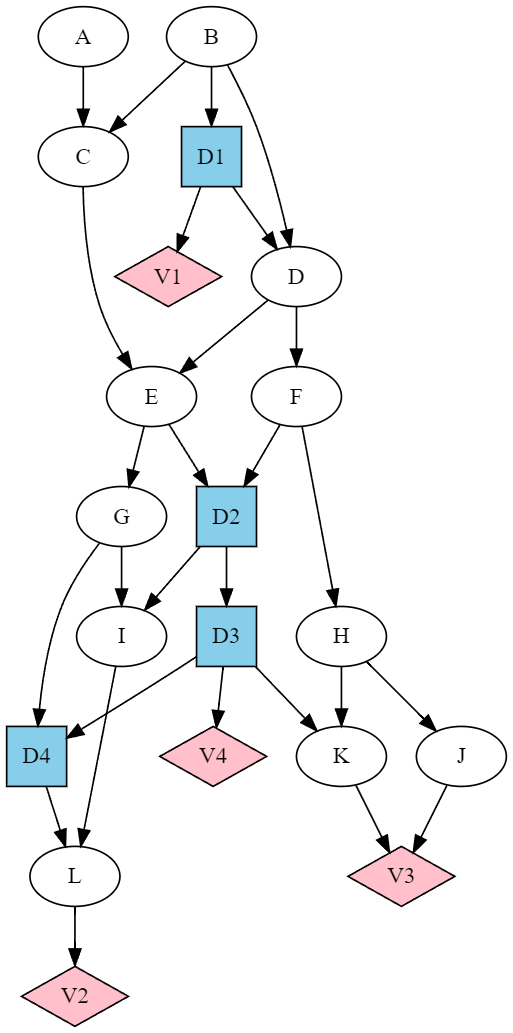
\includegraphics[width=2.3in]{influ-diag/sha-fig1.png}
%\caption{ID example from Ref.\cite{sha-influ-diag}}
%\label{fig-sha-fig1}
%\end{figure}
%
%
%\begin{figure}[h!]
%\centering
%\includegraphics[width=6in]
%{influ-diag/influ-diag-stages.jpg}
%\caption{Different decision stages for the ID shown in Fig.\ref{fig-sha-fig1}.}
%\label{fig-jensen-stages}
%\end{figure}
%
%\begin{figure}[h!]
%\centering
%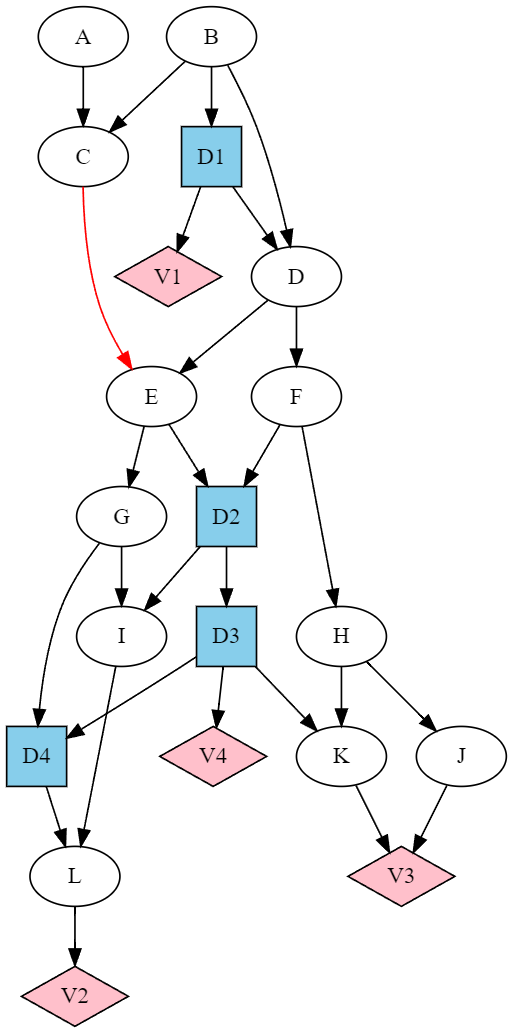
\includegraphics[width=2.3in]{influ-diag/sha-fig1a.png}
%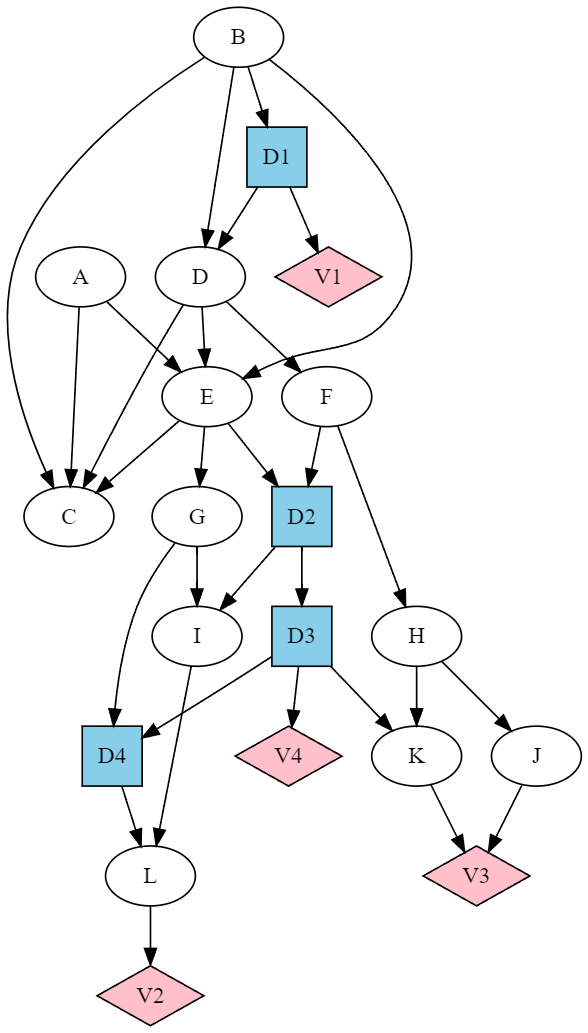
\includegraphics[width=2.3in]{influ-diag/sha-fig1b.png}
%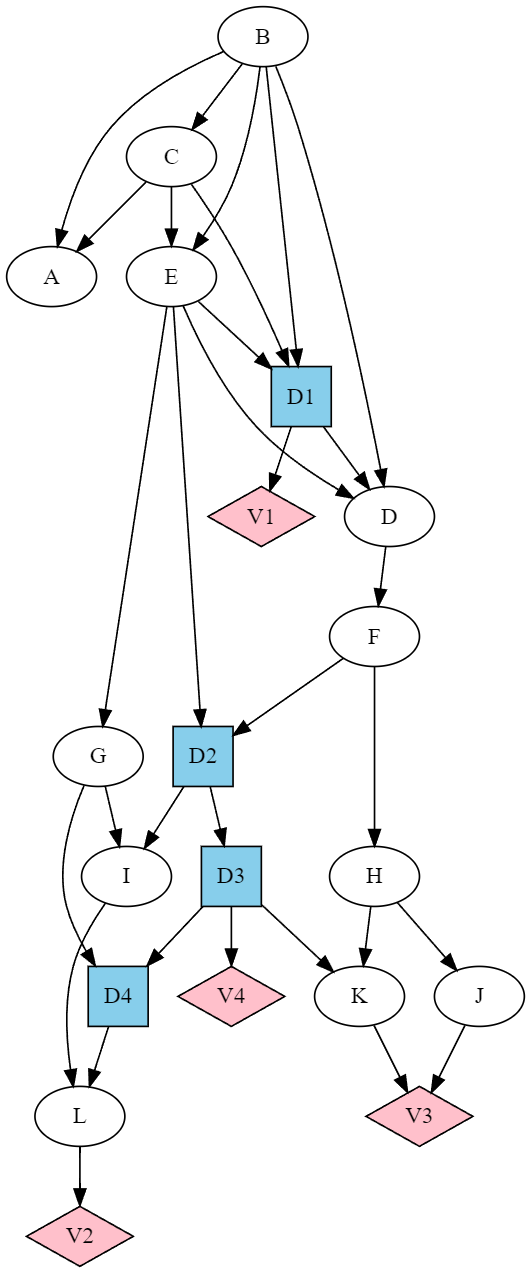
\includegraphics[width=2.3in]{influ-diag/sha-fig1c.png}
%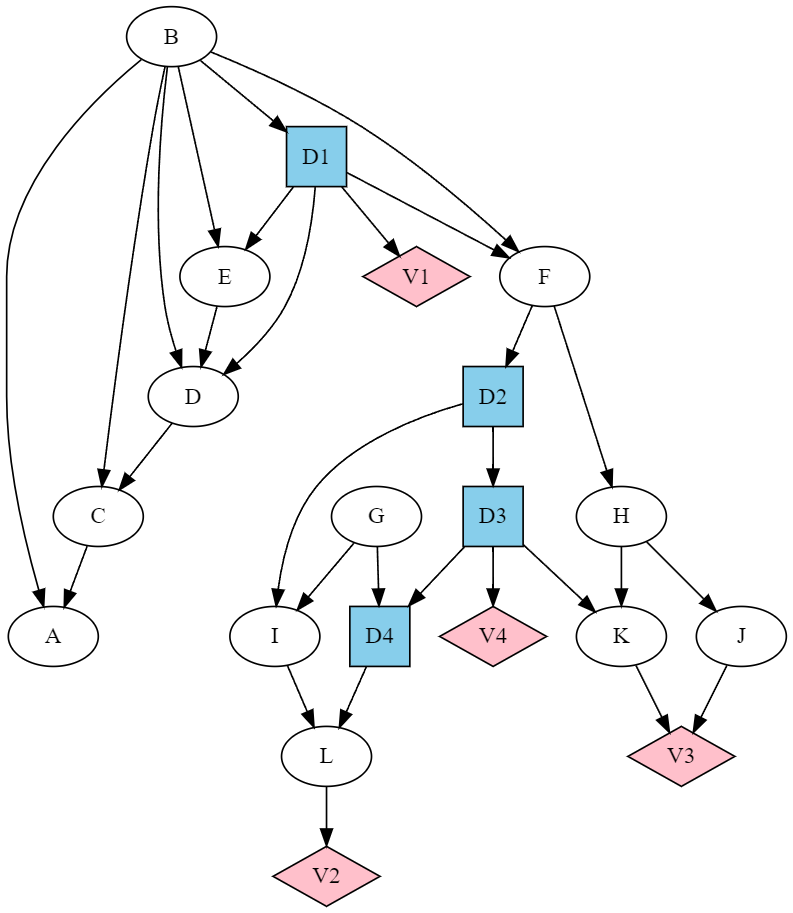
\includegraphics[width=3in]{influ-diag/sha-fig4.png}
%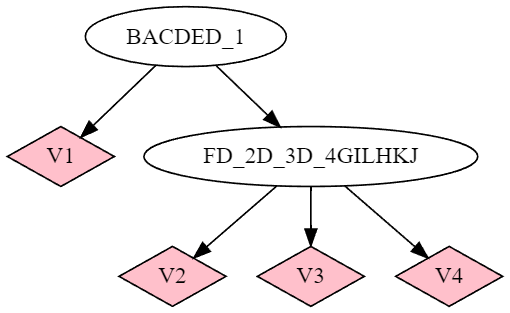
\includegraphics[width=2in]{influ-diag/sha-fig4coarse.png}
%\caption{T=Top, B=Bottom, L=Left, R=Right. {\bf TL:} the ID of Fig.\ref{fig-sha-fig1}. Arrows to be reversed in red.,
%{\bf TR:} the ID of TL after reduction to requisite
%observations. {\bf BL:} the ID of TR after reduction to a tree.
%{\bf BR:} the ID of BL after merging some nodes.}
%\label{fig-sha-fig134}
%\end{figure}
%
%

